%************************************************
\chapter{Konzept}\label{ch:concept}
%************************************************
%

\section{Netzwerk Strukturen}
\todo{Anwendungsfall Analyse? -- evt in Einleitung schieben.}

Im Folgenden wird betrachtet wie die Netzwerkstruktur der Clients im Falle von Slidesync und \schulCloud zusammensetzen.
\subsection{\schulCloud}
Bei der \schulCloud lassen sich im wesentlichen zwei Anwendungsszenarien unterscheiden. Zum einen die Anwendung im Unterricht. Der Lehrer stellt z.B. eine Aufgabe die mit Hilfe der \schulCloud durchgeführt werden soll. Daraufhin besuchen die Schüler die entsprechende Seite und bearbeiten die Aufgabe. In einem kurzen Zeitfenster laden also mehrer Schüler während sie sich im gleichen lokalen Netzwerk befinden, dem der Schule, die selben Inhalte herunter. Bei dem anderen Szenario wird die \schulCloud außerhalb des Unterrichts genutzt. Z.B. bereitet der Lehrer den Unterricht vor oder die Schüler bearbeiten gestellte Hausaufgaben. Die Nutzer befinden sich nicht zwangsläufig im selben Netzwerk. Auch Laden die Nutzer die selben Daten nicht notwendigerweise in einem kurz Zeitfenster sondern verteilt über einen längeren Zeitraum. Es findet jedoch auch keine so starke Auslastung des Netzwerks statt. Deshalb wird im Rahmen dieser Arbeit vor allem das erste Szenario betrachtet.

\subsection{Slidesync}
Die Verteilung der Clients auf Netzwerke kann sich bei Slidesync von Event zu Event stark unterscheiden. Da sich Slidesync jedoch hauptsächlich für Streams von mittleren bis großen Unternehmen wendet, lässt sich beobachten das viele der Nutzer sich gemeinsam in einem lokalen Netzwerk, einem Standort, befinden. Um die Last der Unternehmensnetzwerke zu reduzieren, werden bei einigen Unternehmen caching Server eingesetzt. Betrachtet man 10 Events mit caching Infrastruktur im Internen netz stellt man fest das 64\% der Teilnehmer aus dem internen Netz \todo{caching erklären} auf das Event zugegriffen haben. In dieser Arbeit wird betrachtet wie die Last auf das interne Netz reduziert werden kann ohne das zusätzliche caching Server eingesetzt werden müssen.

\subsection{Gemeinsamkeiten}

\begin{itemize}
	\item 
\end{itemize}

\section{Architektur}

Schul und Unternehmens Netzwerke sind meistens so aufgebaut das viele Clients über einen oder mehrere WAN Anbindungen mit dem Internet verbunden sind. Werden Ressourcen geladen müssen diese über das WAN geladen werden. Dies ist in der Regel auch der Fall wenn mehrere Clients die selben Ressourcen benötigen. Abbildung \ref{fig:school} zeigt den typischen Aufbau eines solchen Netzwerks. Übersteigt die benötigte Bandbreite der Clients die der durch as WAN zur Verfügung gestellten, so kommt es zu mitunter sehr teuren Netzwerk Ausfällen die ganze Unternehmensstandorte betreffen können. Durch die dadurch resultierenden langen Ladezeiten kann es zu einer starken Einschränkung des Nutzererlebnisses und der Nutzerzufriedenheit kommen.\cite{userWaitingTime} Um dem entgegen zu wirken wird versucht mit caching Appliances den Datenverkehr der über das Internet geladen werden muss zu reduzieren. Slidesync z.B. bietet dazu Unternehmen ein eigenes lokales CDN an bei dem Server in dem Netzwerk betrieben werden. Dies verursacht jedoch kosten und Konfigurationsaufwand. Damit eigenen es sich nur für größere Unternehmen die den Service häufig nutzen.

\begin{figure}[!h]
	\centering
	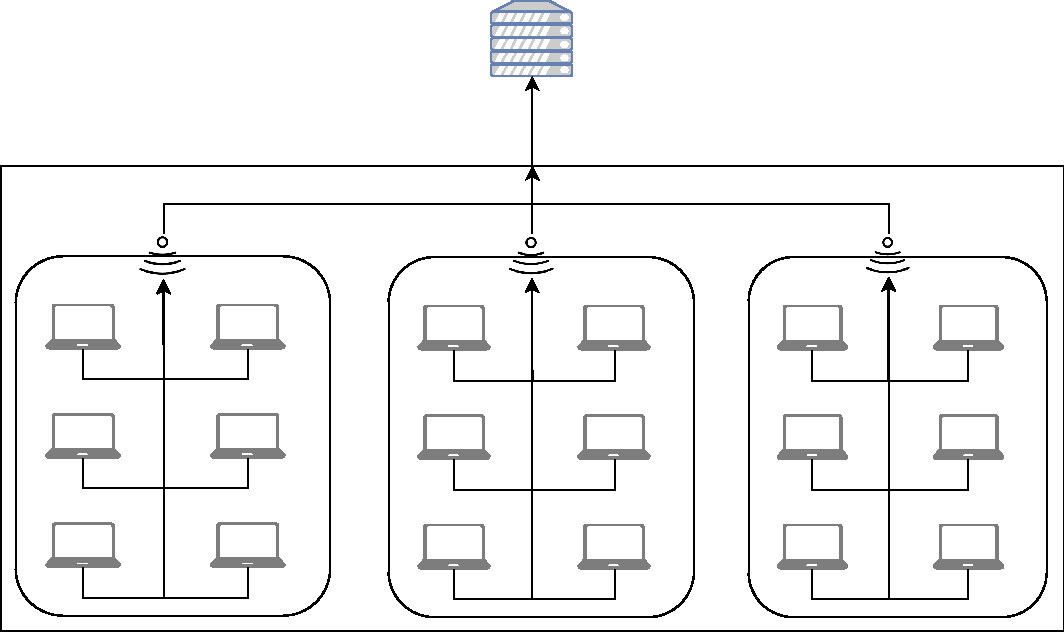
\includegraphics[width=0.8\textwidth]{figures/network_current}
	\caption[A Figure Short-Title]{Netzwerkverkehr in einem herkömmlichen Netzwerk}
	\label{fig:school}
\end{figure}

In den betrachteten Anwendungsfällen besteht eine hohe zeitlich und inhaltliche Lokalität der Daten. Dies kann genutzt werden um die benötigte Bandbreite zu reduzieren. Dazu soll im Folgenden eine interne Verteilung mittels eines hybriden \pTp CDNs untersucht werden. Abbildung \ref{fig:mesh} zeigt exemplarisch den Aufbau eines solchen Netzwerkes. Anstatt das jeder Client sich die Ressource von einem externen Server lädt, lädt nur noch ein Nutzer je Subnetz die Resource über das WAN. Dieser verteilt die Resource dann im internen Netzwerk an andere Clients die diese dann ebenfalls wieder bereitstellen.

Benötigt ein Client eine Resource versucht er zunächst die Resource über sein \pTp Mesh zu laden. Ist dies nicht möglich lädt er sie über einen externen Server. Hat ein Peer eine Resource geladen speichert er sie zwischen und stellt sie für andere Clients bereit.

\begin{figure}[!h]
	\centering
	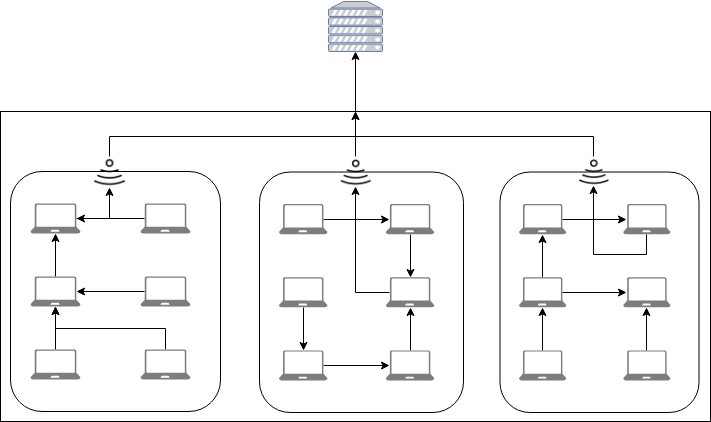
\includegraphics[width=0.8\textwidth]{figures/network_p2p}
	\caption[A Figure Short-Title]{Netzwerkverkehr in einem Peer To Peer CDN}
	\label{fig:mesh}
\end{figure}

Da sowohl im Kontext der Schule als auch bei Unternehmen kein Wissen im Bereich der Computer Administration seitens der Nutzer vorausgesetzt werden kann, muss ein Ansatz gewählt werden der keine Installation auf Seiten der Nutzer benötigt.

Um dies zu erreichen wird eine Kombination aus Webrtc und Service Workern verwendet. Der Javascript Code lässt sich als ein Plugin einbinden und erfordert nur geringen Konfigurationsaufwand seitens der Anwendungsentwickler. Da sich die Art der Seitennutzung von Anwendung zu Anwendung jedoch stark unterscheidet muss das Peer Meshing serverseitig für jede Anwendung geschrieben werden. So kann Domainenspezifisches wissen ausgenutzt werden um eine bessere überlappung der von den Clients benötigten Ressourcen zu erreichen. 

Die eingesetzte Technologie zur Übertragung von Daten zwischen Browsern ist WebRTC. WebRTC ist ein offener Standard und ermöglicht es Browser paarweise zwecks Datenaustausch zu verbinden. Der große Vorteil dieser Technologie ist, dass sie direkt von modernen Browsern unterstützt wird, wodurch keine zusätzliche Software installiert werden muss. Konkret werden Webrtc DataChannel genutzt.

Für den Datenaustausch müssen wechselseitig DataChannel zueinander aufgebaut werden. Die Ausgangslage ist, dass die Peers wissen, dass es den anderen gibt, aber nicht wie der jeweils andere zu erreichen ist. Um diese Problematik zu lösen, existiert ein Vermittlungsserver (Signaling server).

Als erstes werden Informationen, über die Verbindung die aufgebaut werden soll, an den Signaling server gesendet. Es wird ein SDP-Offer gesendet(SDP für Session Description Protocol). Dieses SDP-Offer leitet der Signaling server an die Peers in dem selben Mesh sind weiter. Geantwortet wird mit einer SDP-Answer, welche Informationen über die abgestimmte Verbindung enthält und über den Signaling server zurück geleitet wird.

Damit eine direkte Verbindung aufgebaut werden kann, müssen über den Signaling server noch weitere Informationen wie ICE-Kandidaten ausgetauscht werden. ICE steht hierbei für Interactive Connectivity Establishment und ist fester Bestandteil von WebRTC. Es ist für den Aufbau der Browser-zu-Browser-Verbindung verantwortlich. ICE-Kandidaten enthalten hauptsächlich Informationen darüber wie ein bestimmter Nutzer erreichbar ist (also z.B. private oder öffentliche IP-Adresse). Ermittelt werden diese ICE-Kandidaten mithilfe eines STUN-Servers und dem dazugehörigen Session Traversal Utilities for NAT (STUN) Protokoll. Wie der Name des Protokolls schon verrät, wird es vor allem benötigt um auch Nutzer erreichen zu können die keine eigene öffentliche IP-Adresse besitzen, bei denen also Network Address Translation (NAT) eingesetzt wird. Dies ist aufgrund der mangelnden Anzahl an IPv4-Adressen bei fast jedem Internetnutzer der Fall.

% herausstellen das ein plugin entwickelt wird das eingebunden werden kann
%Die eingesetzte Technologie zur Übertragung von Daten zwischen Browsern ist WebRTC. WebRTC ist ein offener Standard und ermöglicht es Browser paarweise zwecks Datenaustausch zu verbinden. Der große Vorteil dieser Technologie ist, dass sie direkt von modernen Browsern unterstützt wird, wodurch keine zusätzliche Software installiert werden muss. Konkret wird von uns ein sog. DataChannel genutzt.
%
%Für den Datenaustausch müssen wechselseitig DataChannel zueinander aufgebaut werden. Die Ausgangslage ist, dass die Peers wissen, dass es den anderen gibt, aber nicht wie der jeweils andere zu erreichen ist. Um diese Problematik zu lösen, existiert ein Vermittlungsserver (Signaling server).
%
%Als erstes werden Informationen, über die Verbindung die aufgebaut werden soll, an den Signaling server gesendet. Technisch wird ein SDP-offer gesendet, wobei SDP für Session Description Protocol steht. Dieses SDP-offer leitet der Signaling server an die Schüler in der Klasse/Schule weiter. Geantwortet wird mit einer SDP-answere, welche Informationen über die abgestimmte Verbindung enthält und über den Signaling server zurück geleitet wird.
%
%Damit eine direkte Verbindung aufgebaut werden kann, müssen über den Signaling server noch weitere Informationen wie ICE-Kandidaten ausgetauscht werden. ICE steht hierbei für Interactive Conectivity Establishment und ist fester Bestandteil von WebRTC. Es ist für den Aufbau der Browser-zu-Browser-Verbindung verantwortlich. ICE-Kandidaten enthalten hauptsächlich Informationen darüber wie ein bestimmter Nutzer erreichbar ist (also z.B. private oder öffentliche IP-Adresse). Ermittelt werden diese ICE-Kandidaten mithilfe eines STUN-Servers und dem dazugehörigen Session Traversal Utilities for NAT (STUN) Protokoll. Wie der Name des Protokolls schon verrät, wird es vor allem benötigt um auch Nutzer erreichen zu können die keine eigene öffentliche IP-Adresse besitzen, bei denen also Network address translation (NAT) eingesetzt wird. Dies ist aufgrund der mangelnden Anzahl an IPv4-Adressen bei fast jedem Internetnutzer der Fall.
%
%In dem Signaling server selbst wird die Logik abgebildet, wie die Klassen und Schüler miteinander in Verbindung stehen. Implementiert wurde dieser mit socket.io, da die native Klassenorganisation und Websocket-Technologie sich nahezu perfekt für unser Szenario anbot.

% schon geschrieben:
%Genereller Architektur Ansatz
% interne verteilung in subnetzen vs wan verbindung
% Klassische Server architekur mit client und server beschreiben + bild
% p2p mit bild zeigen netzarchitektur
% kommunikation zwischen peer anhand von vereinfachter architektur beschreiben
%	bild peer to peer zwischen browsern ohne service worker
%	peer to peer zwischen browsern
% hybrid p2p CDN ansatz
% keine installation auf clientseite
% domainen wissen soll genutzt werden um clients zu verbinden
% 
%
%
%


%bild schule wie in blockpost?
%
%
%%

% "hybrid p2p cdn"
%konfiguration von subnetzen?
\begin{figure}[!h]
	\centering
	\includegraphics[width=0.8\textwidth]{figures/service_worker_app}
	\caption[A Figure Short-Title]{Service Worker - Webrtc}
	\label{fig:mesh}
\end{figure}

%\begin{itemize}
%	\item Browser based without plugin
%	\item einfache einbindung
%	\item Server architektur diagram --> Server, Stun, CDN, P2P CDN
%	\item Discussion verschiedener Request interception techniken
%	\item Special Tags
%	\item http interceptor
%	\item 	only ajax calls
%	\item 	erst wenn seite komplett geladen
%	\item Browser Plugins
%	\item evtl coporate cdn erwähnen
%	\item extra software auf client
%	\item Service Worker -- > WEBRTC
%	\item Script für execution
%	\item Webrtc - Datachannel
%	\item Service worker cached request
%	\item warum service worker
%	\item 	vergleich anderer Ansätze
%	\item 	Literatur anschauen
%\end{itemize}
%	\item 	https://developer.mozilla.org/en-US/docs/Mozilla/Add-ons/WebExtensions/Intercept_HTTP_requests
%Für unsere Implementation wird für das Zwischenspeichern von Daten ein Serviceworker eingesetzt. Serviceworker können wie ein Proxy zwischen dem Webbrowser und dem Webserver agieren, welcher die Webseite bereitstellt. Stellt ein Browser eine Anfrage, so wird diese vom Serviceworker abgefangen. Der Serviceworker schaut zunächst in seinem Cache, der sog. IndexDB, ob er die gestellte Anfrage beantworten kann. Ist dies nicht der Fall, so wird die Anfrage an den Webserver weitergeleitet. Wird die gleiche Anfrage nochmals gestellt, kann diese aus dem Cache beantwortet werden, da gestellte Anfragen eine gewisse Zeit lang zwischengespeichert werden.
%\begin{figure}[!h]
%	\centering
%	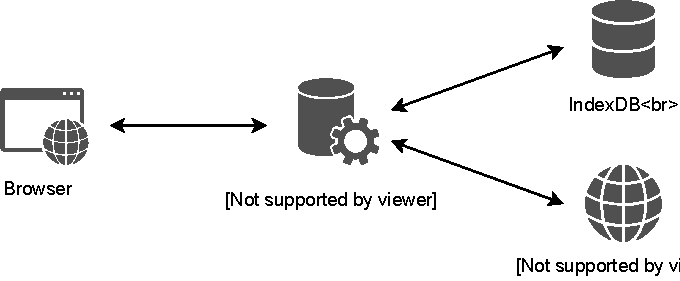
\includegraphics[width=0.8\textwidth]{figures/ServiceWorker}
%	\caption[A Figure Short-Title]{A Figure Title}
%	\label{fig:sequenceDiagram}
%\end{figure}
%
%

\section{Javascript Proxies - Abfangen von Anfrage}

Damit ein Client-seitiges \cdn möglich ist, ist es notwendig das die Abfragen des Browsers abgefangen und auf anderem Weg beantwortet werden können. Nachdem der Browser nach einer Anfrage URL augelöst hat(DNS-lookup) lädt er die abgefragte Seite. Ist die Seite geladen beginnt der Browser die im HTML Dokument verlinkten Dokumente zu laden. Das sind neben Bildern auch CSS und Javascript Dateien. Ein CDN muss in der Lage sein auf all diese Anfragen reagieren zu können.

\begin{figure}[!h]
	\centering
	\includegraphics[width=0.8\textwidth]{figures/browser_abfrage}
	\caption[A Figure Short-Title]{Ablauf einer HTML abfrage im Browser}
	\label{fig:browser_abfrage}
\end{figure}


Um dies zu realisieren gibt es verschiedene Möglichkeiten. Turbolinks unterbricht die Weiterleitung nachdem ein Link angeklickt wurde und lädt die abgefragte Seite mit Ajax. Dadurch ist es möglich die zu zeichnenden Elemente selbst auszuwählen und manuell teile der Seite zu cachen. Dieser Ansatz ließe sich auch für ein \cdn verwenden. Allerdings ist es nötig die Javascript Page load Events durch eigene Events zu ersetzen und bestimmte Teile des Javascript Codes umzuschreiben. Javascript Code wird bei diesem Ansatz nach Navigation auf eine neue Seite nicht neu geladen. Auch wenn dies die Ladezeiten verringert ist eine Integration ohne Anpassung des Anwendungscodes nicht möglich. Ebenfalls ist es nicht möglich Anfragen abzufangen die beim ersten Besuch der Seite entstehen, sondern nur solche die nach weiterer Navigation entstehen.

Eine weitere Möglichkeit besteht darin eigene HTML tags einzuführen und diese nachdem die eigentliche Seite und das \cdn script geladen wurde mit Ajax nachzuladen. Dadurch lässt sich mit Javascript kontrollieren woher die Ressource geladen werden soll. Allerdings können Ressourcen die über das \pTp CDN geladen werden sollen erst geladen werden wenn das komplette HTML Dokument und das \cdn script geladen sind. Dies kann die Ladezeiten beeinflussen und ebenfalls Anpassungen im Javascript Code der Anwendung notwendig machen. Wird in einer nachgeladenen Javascript Datei ein Eventhandler auf ein Event registriert das bereits gefeuert wurde, so wird dieser Code nicht mehr ausgeführt. 

Service Worker sind eigene Prozesse die in einem anderen Kontext laufen als die eigentliche Webseite. Einmal registriert existieren sie und fungieren als proxy, unabhängig davon ob die Webseite gerade geladen ist oder nicht. Besucht ein Nutzer die Seite wird der Service Worker geladen. Kehrt er wieder so ist der Service Worker bereits aktiv und kann Anfragen des Browsers abfangen. Da einer der Anwendungsfälle für Service Worker das Offline verfügbar machen von Webanwendungen ist, verfügen sie über Unterstützung von Caching-APIs. Durch die Caching-API ist es möglich Anfragen zu speichern und zu einem späteren Zeitpunkt wieder abzurufen. Somit ist es nicht nur möglich eigene Anfragen aus dem Cache zu beantworten, sondern ebenfalls gespeicherte Ressourcen an andere Clients auf Anfrage weiter zu leiten. Daher eigenen sie sich gut für die Verwendung als Proxy in einem Clientseitigen \cdn.   

%\begin{itemize}
%	\item request Reihenfolge
%	\item https://vanseodesign.com/web-design/browser-requests/
%	\item html dokument
%%	\item script tags
%	\item bilder
%	\item js wird geladen
%	\item wie als requests die als script tag eingebunden werden abfangen?
%	\item abfangen mit jsavascript event im page context nicht möglich
%	\item kein handler
%	\item durch timing unmöglich
%	\item turbolinks verhindert page load und mach anfragen per ajax
%	\item - mit eigenen tags späteres manuelles laden von ressourcen möglich
%	\item - hoher anpassungsbedarf auf anwendungsseite...
%	\item websockets
%	\item eigener Prozess
%	\item sind zur ladezeit der seite bereits verfügbar
%\end{itemize}

\section{Verbinden von Peers - Signaling}
Um eine Verbindung zwischen den Peers aufzubauen ist ein Signaling Process erforderlich. Der Webrtc Standard schreibt nicht vor wie das Signaling durchgeführt werden soll, jedoch bieten sich hierzu Websockets an, da eine bidirektionale Kommunikation notwendig ist. Da das Schul-Cloud backend in Nodejs und Slidesync in Ruby on Rails programmiert sind biete es sich an eine websocket Implementierung zu wählen die für beide Backends Schnittstellen anbietet. Faye\footnote{https://faye.jcoglan.com/} bietet neben Einem Browser-Client auch Backend Clients für verschiedene Programmiersprachen, darunter auch Nodejs und Ruby an. 
\begin{figure}[!h]
	\centering
	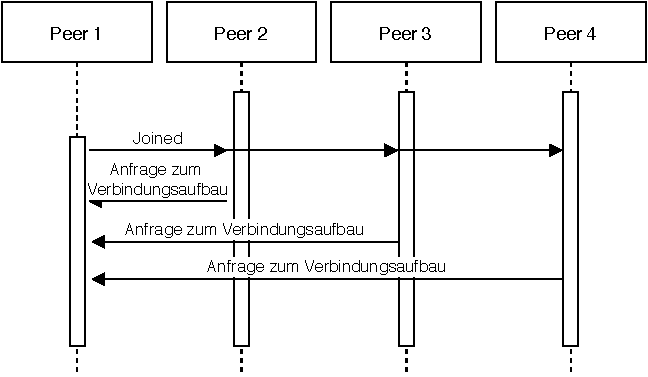
\includegraphics[width=0.8\textwidth]{figures/Signaling}
	\caption[A Figure Short-Title]{Signaling Ablauf}
	\label{fig:mesh}
\end{figure}

Tritt ein Client einem Peer Mesh bei, so sendet er eine Nachricht mit seiner eigenen PeerId auf einen Websocket channel({Prefix}/joined). Alle Peers des Meshes sind auf diesem Websocket Channel registriert und empfangen die Nachricht. Empfängt ein Peer die Nachricht das ein neuer Peer dem Netzwerk beigetreten ist, beginnt er eine Webrtc Verbindung zu dem Peer aufzubauen.

\begin{figure}[!h]
	\centering
	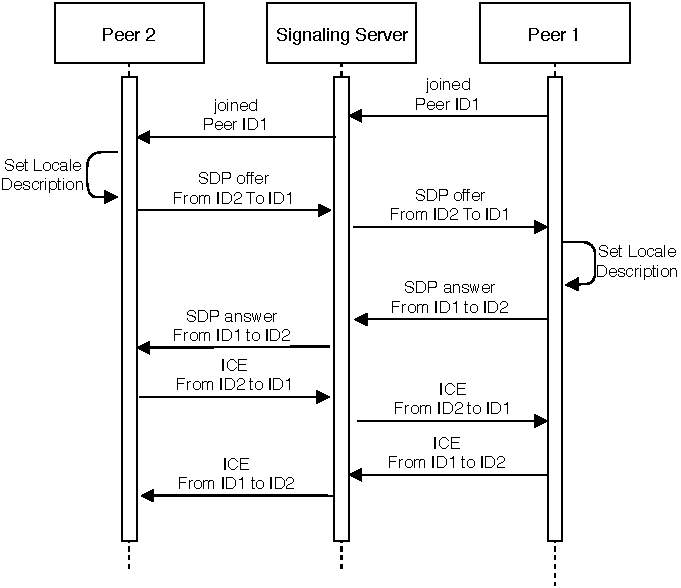
\includegraphics[width=0.8\textwidth]{figures/Signaling-Webrtc}
	\caption[A Figure Short-Title]{Ablauf Verbindungsaufbau}
	\label{fig:signaling-connection}
\end{figure}

Abbildung \ref{fig:signaling-connection} zeigt den Verbindungsaufbau zwischen zwei Peers. Nachdem Peer1 über den Websocket Channel mitgeteilt hat das er dem Peer Mesh beitreten will sendet Peer2 ein SDP-Offer über einen Websocket Channel zu Peer1. Dazu registriert sich Peer1 auf dem Channel '{Prefix}/{ClientId}' über den er für Peer2 erreichbar ist. Hat Peer1 das SDP-Offer erhalten sendet er ein SDP-Answer zurück. Mit den dadurch erhaltenen Informationen tauschen die beiden Clients nun ICE Pakete über den Websocketchannel aus. Im Anschluss können beide Clients über Webrtc direkt miteinander kommunizieren. 

Verlässt ein Client das \pTp Netzwerk so müssen die andern Clients darauf reagieren und ihn aus ihrer Liste von Peers löschen. Zwar wäre es möglich eine Nachricht im Falle das ein Client die Seite verlässt zu senden, z.B. mittels dem onbeforeunload\footnote{https://developer.mozilla.org/en-US/docs/Web/API/WindowEventHandlers/onbeforeunload} Javascript Event, jedoch ist dies sehr unzuverlässig. Im Falle das der Client z.B. die Internetverbindung verliert oder der Computer ausgeschaltet wird kann dieses Event nicht mehr ausgelöst, und somit auch keine Nachricht mehr an die Peers gesendet werden. Daher beobachten die Peers den Status des Webrtc Datachannels. Ändert er seinen zustand zu geschlossen so wird der Peer aus dem Netzwerk entfernt. Auf diesem Weg können fehlerhafte Peers entfernt werden ohne darauf angewiesen zu sein das sie im Fehlerfall noch in der Lage sind eine Nachricht an die anderen Peers zu senden.

%\begin{itemize}
%	\item Signaling
%	\item faye
%	\item über Websocket channel
%	\item Websockets werden verwendet um Verbindungen aufzubauen
%	\item Danach Webrtc zum direkten herstellen der Verbindung
%	\item Anwendungslogick
%	\item Signaling over Kademlia
%\end{itemize}

\section{Mesh Zuordnung}
Im Folgenden werden verschiedene Zuordnungsstrategien zur Bildung von Peer Meshes diskutiert. Dazu wird der typische Workload beider Anwendungen analysiert um eine jeweils geeignete Strategie zu wählen. 

- Vergleich von Meshing verfahren/peer routing aus Literatur
\subsection{Routing}
Im Folgenden werden verschiedene Routing \pTp Routing Algorithmen aus der Literatur vorgestellt und diskutiert welcher Ansatz für die betrachteten Anwendungsfälle am geeignetsten ist.

\begin{itemize}
	\item Datenstruktur
	\item  Dezentralisierte Datenspeicherung
	\item Daten werden über SPeicherknoten verteilt
	\item Jeder Knoten Eintrag in Hashtabelle
	\item direct storage: Daten in Hashtabelle
	\item nur für kleine Daten
	\item indirect storage: Verweis auf daten in Hashtabelle
	\item Eigenschaften:
Fehlertoleranz
Lastenverteilung
Robustheit
Selbstorganisation
Skalierbarkeit
	\item consistent hashing
	\item Server zum routen
https://www.coralcdn.org/pubs/
\end{itemize}

\begin{itemize}
	\item Rechnung Peersuche laufzeit:
	\item Verbinden von 2Peers ohne Netzlaufzeit: 30ms
	\item Angenommene Latenz: round trip: 50ms
	\item 80ms
	\item 80*4 = 320ms
	\item Log(1000) = 3 + 1 
	\item 4 Verbindungen müssen aufgebaut werden
\end{itemize}

\subsubsection{Chord}

How to save files in advance???
save file references
\subsubsection{Kademlia}
\subsubsection{IPFS}
\subsubsection{Kelips}
\subsubsection{Pastry}
\subsection{\schulCloud}
Analyse workload mit grafik

\begin{itemize}
	\item Schulcloud
	\item 	
\end{itemize}
Schulcloud
- Global
einfache umsetzung
Kurs unabhänige assets können geteilt werden
Maximale Mesh größe
Mehrere Meshes nötig
Möglicherweise nicht im Mesh mit relevanten Peers
Maximiert die Anzahl der Peers pro Mesh
Wahrscheinlichkeit für selbes Subnetz eher gering
Funktioniert auch mit wenigen Clients
Ineffektiv wenn viele Clients vorhanden sind

- Schule
Einfache Umsetzung
Funktioniert auch mit wenigen Clients
Relativ hohe trefferrate da schulen selten mehr als 1000 Schüler hat
Max mesh größe um die 256(Chrome)
Relativ wahrscheinlich gleiches Subnetz

- Kurs
Hohe trefferrate
Kleine Meshes
benötigt mehr Clients
Relativ wahrscheinlich gleiches Subnetz --> Daten die das bestätigen

hybride Ansätze:
Zwei priorisierte Meshes Schule und Klasse

Berechnung eines Scores für jeden Peer:
Möglichst viele gemeinsame kurse
Liste von Kursen für jeden Peer
Schnittmenge für jeden peer der online ist bilden
Kardinalität der Menge = Score von Peer
Rechenaufwendig Aber machbar
Beste Trefferrate
Funktioniert wenn wenige und wenn viele Peers anwesend sind

\subsection{Slidesync}
Slidesync ist eine Plattform deren Nutzung stark durch die durchgeführten live Events dominiert wird. Ein Moderator erstellt das Event lädt die notwendigen Assets, z.B. Foliensätze, hoch. Live Events werden für eine bestimmte Zeit festgesetzt und Teilnehmer laden zum Start des Events die Seite.\todo{Grafik visits} Ein Großteil des entstandenen Traffics besteht aus HLS Videoseqmenten. Jeder Teilnehmer eines Events benötigt die selben Inhalte.\todo{Grafik traffic} 

Die Peer Meshes in Slidesync werden als voll vermaschte Netzte abgebildet. Da alle Teilnehmer eines Events zu großen Teilen die selben Daten benötigen können sie in dem selben Mesh untergebracht werden. Um zu gewährleisten das sich die Peers im Selben Subnetz befinden teilen sich nur solche ein Peer Mesh die sich in der Selben IP Range befinden. Ein weiterer wichtiger Factor ist der Kommunkationsmehraufwand der durch das halten von Verbindungen zu vielen Peers entsteht. Deshalb ist es nicht möglich bei größeren Events alle Peers im selben Peer Mesh unter zu bringen. Deshalb werden Sub Meshes gebildet in denen sich eine maximale Anzahl an Peers befinden können. 

Abbildung \ref{fig:mesh-slidesync} zeigt eine beispielhafte Aufteilung von Peer Meshes für ein Event. Für Netzwerk A und B werden jeweils zwei Meshes erzeugt und nur solche Clients werden miteinander verbunden die sich auch im Selben Subnetz befinden. Jedes Netzwerk wird wiederum in zwei Sub-Meshes unterteilt.

\begin{figure}[!h]
	\centering
	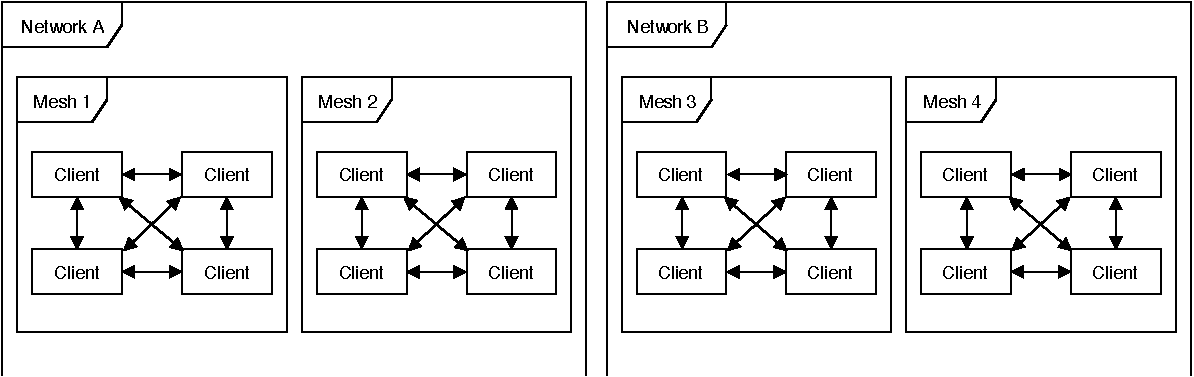
\includegraphics[width=0.8\textwidth]{figures/slidesync_peer_meshes}
	\caption[A Figure Short-Title]{Peer to Peer Meshes - Slidesync}
	\label{fig:mesh-slidesync}
\end{figure}

Um sicherzustellen das ein Peer sich auch aktiv am Mesh beteiligen kann sendet er regelmäßig ping Nachrichten an den Server. Da dieser Mechanismus in Slidesync schon zu vor zur Erhebung von Statistiken verwendet wurde, wird diese Nachricht lediglich um den Zustand des \cdns erweitert. Meldet ein Peer sich nicht innerhalb einer Minute oder meldet er das eine Verbindung zum \pTp Netzwerk nicht möglich ist, so wird er als nicht mehr mit dem \pTp \cdn verbunden betrachtet. Sind alle aktuell verfügbaren Peer Meshes voll, so wird ein neues Peer Mesh angelegt und ein Hintergrund Job gestartet der alle Peer die als nicht verbunden betrachtet werden aus den Peer Meshes entfernt und die Meshes wieder als verfügbar markiert. Dadurch wird die Beantwortung der aktuelle Anfrage nicht verzögert und der Hintergrund Job nur bei Bedarf gestartet. Ebenso werden so Peers aussortiert deren Browser das \pTp \cdn nicht unterstützen, da der Anwendungsserver darüber zum Zeitpunkt der Zuordnung noch keine Kenntnis darüber hat.
%
%\begin{itemize}
%	\item Aussortieren von alten peers
%	\item Background Job
%	\item Job wird gestartet wenn kein freies Mesh verfügbar ist
%	\item Peers senden regelmäßig ping an server
%	\item Kommt ping nicht mehr wird angenommen Peer das Peer offline ist
%	\item Unterstützt ein Peer Browser das CDN nicht wird kein Ping mehr gesendet
%\end{itemize}
%Analyse workload
%
%Live Streaming
%- Event basiert
%- interessante Inhalte zum Teilen: Video stream
%- Viele Nutzer pro Event seite
%- aufsplittung von Peers anhand von lokalen Netzwerken wenn verfügbar

% voll vermaschtes netz
% mit bild
% Nutzung des anwendungswissens
% ip subnetz plus gleicher Kurs/stream


\section{Routing - finden von Ressourcen}

Um das \pTp Netzwerk als \cdn Nutzbar zu machen ist es wichtig das ein Peer in der Lage ist herauszufinden wer welche resource bereitstellt.

%DHT\todo{distributed hash tables erklären}
%
%Structured vs untructured

Da das Routing von Ressourcen bei den Betrachteten Anwendungsfällen in einem Zeitkritischen Moment erfolgen muss wurde sich für einen anderen Ansatz entschieden. Jeder Peer hält eine Hashtabelle mit den Ressourcen seiner Peers vor. Fügt ein Peer eine neue Ressource zu seinem Cache hinzu oder entfernt sie muss er alle verbundenen Peers über diese Änderung informieren. Dadurch muss im Falle einer Anfrage nicht erst die Ressource im Netzwerk gesucht werden. Dies ist möglich durch die Struktur des Netzwerkes. Da nicht alle Peers miteinander verbunden sind sondern voll vermaschte sub-meshes gebildet werden ist es möglich alle relevanten Peers über Änderungen zu informieren. Dadurch ist es möglich die Rechenleistung für das auffinden von Ressourcen in einen weniger Zeitkritischen Moment zu verlagern. Jedoch hat dies zur Folge das die Meshes so gebildet werden müssen das die Peers möglichst viele Ressourcen gemeinsam benötigen. Ist eine Ressource nicht im Mesh vorhanden wird sie vom Server geladen. 

%\begin{itemize}
%	\item 
%\end{itemize}

\todo{Duplicate}
%Structured vs unstructured networks
%
%Kollaborative File Sharing Protokolle wie z.B. Bitorrent verwenden häufig verteilte Hashtabellen zum auffinden von Ressourcen im Netzwerk. 
%Zhang proposed a DHT based P2P resource pool, SOMO
%[22], [23] to manage global resources and optimize multiple
%ALM (Application Layer Multicast) sessions,

%server hält liste vor --> kommunikation mit server nötig. \study
%
%peer fragt im Netzwerk an --> mehr kommunikation wenn in zeitkritischem moment \study
%
%peer halten liste von requests aktuell. Kommunikationsoverhead in zeitunkritischem moment \study
%	 peer weiß immer bei wer welche resource hat

% evtl diskussion verschiedener methoden 
%   server hält liste vor --> kommunikation mit server nötig
% peer fragt im Netzwerk an --> mehr kommunikation wenn in zeitkritischem moment
% peer halten liste von requests aktuell
%    kommunikationsoverhead in zeitunkritischem moment
%	 peer weiß immer bei wer welche resource hat
% am Anfang wird die zuordnung von einem peer an den neuen geschickt

\subsection{ Updates }
\begin{figure}[!h]
	\centering
	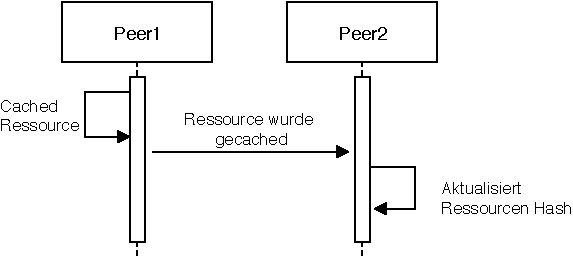
\includegraphics[width=0.8\textwidth]{figures/Ressourcen_update}
	\caption[A Figure Short-Title]{Flussdiagramm Ressourcen Update}
	\label{fig:update_resource}
\end{figure}

Lädt ein Client eine neue Ressource in den Cache oder löscht er eine aus dem Cache so muss er seinem Peer Mesh dies mitteilen. Dazu sendet er eine Nachricht an alle Peers mit denen er verbunden ist. Die Kommunikation findet über den zuvor geöffneten Webrtc Datachannel statt. Empfängt ein Peer ein Update von einem anderen Peer so ändert er entsprechend die gespeicherte Hashmap von Ressourcen für diesen Peer.

%\begin{itemize}
%	\item Diagramm
%	\item Client lädt ressource 
%	\item Client cached Resource
%	\item Sendet nachricht an peers das Resource gecached wurde und verfügbar ist
%	\item Clients speicher Client Resource hash in Hashmap
%
%\end{itemize}
\subsection{Subnetzerkennung}

Um Sicherzustellen das nur Peers aus dem gleichen lokalen Netzwerk miteinander verbunden werden muss eine Subnetzerkennung implementiert werden.
Um dies zu erreichen gibt es im wesentlichen zwei Wege. Zum einen kann, wenn die IP-Range des Unternehmensstandorts/der Schule bekannt ist diese genutzt werden um nur jene Peers in einem Mesh zu verbinden die sich im selben lokalen Netzwerk befinden. Dazu wird der Netzwerkanteil der IP Adresse mit der des Unternehmens/Schulnetzes verglichen. Stimmt der Netzwerkanteil überein so befinden sie sich im Schul- bzw. Unternehmensnetz. 

Alternativ kann auch auf die Angabe eine NAT-Servers beim Webrtc Verbindungsaufbau verzichtet werden. Dadurch ist es Peers die sich hinter einem NAT oder einer Netzwerk Firewall befinden nicht mehr möglich sich mit Peers außerhalb des Netzwerkes zu verbinden, sehr wohl aber mit Peers innerhalb des selben lokalen Netzwerkes. Dies hat den Nachteil das Peers gemeinsam in Meshes sind die sich nicht miteinander verbinden können und im Anschluss aussortiert werden müssen. Jedoch muss im Vorfeld kein wissen über IP-Ranges vorhanden sein. Auch eine Konfiguration ist nicht notwendig. 

Das Vergleichen von IP-Adressen hat den Vorteil das bereits zur Einteilung in die Peer meshes bekannt ist in welchem lokalen Netzwerk sich der Peer befindet. Dadurch können die Peers effizienter in die Meshes eingeteilt werden. Jedoch muss das Subnetz bekannt sein und in der Anwendung konfiguriert werden. Auch muss der Anwendung die IP-Adresse des Clients bekannt sein, was im Fall von Schul-Cloud aus Datenschutzgründen nicht möglich ist.

\section{Wiederverwendbarkeit}
%Plug and play
%Konfigurierbarkeit
%einfaches einbinden in existierende anwendungen über npm
%javascript modul
%support von eigenen oder öffentlichen stun servern
%%Plug and play
\section{Open Source}
\begin{itemize}
	\item evtl. Open source erklären
	\item bereitstellung für die Öffentlichkeit
	\item Welche Lizenz?
\end{itemize}
%was ist open source
%bereitstellung für die Öffentlichkeit
%

\section{Offline Support}
\begin{itemize}
	\item Motivation: Internet in Schulen ist nicht immer verfügbar
	\item wie funktionieren offline webanwendungen
	\item Service Worker
	\item Live Streams: Ausfallsicherheit wird erhöht.
	\item quasi bei design
	\item Resourcen werden gecached und sind offline verfügbar
	\item Tobias arbeit Refernzieren
	\item Übertragung im lokalen Netzwerk möglich wenn verbindung aufgebaut ist
	\item Signaling müsste in lokalem netzwerk sein z.b. Rechner vom Lehrer
	\item signaling könnte über webrtc erfolgen z.b. über 
	\item kademlia routing indem Peers als vermittler fungieren
	\item 	evt. browser plugin
	\item 	Wie das routing machen?
	\item Offline scenario:
	\item 	Lehrer Lädt ressourcen vor und macht sie für schüler verfügbar
	\item 	Kein Internet vorhanden
	\item 	Schüler laden Ressourcen von Lehrer
\end{itemize}

\section{Security}
\begin{itemize}
	\item Owasp
%	\item https://www.owasp.org/images/9/90/OWASP_Top_10-2017_de_V1.0.pdf
	\item IP Leak möglich
	\item Stun Server kann nach IP Adresse fragen
	\item Über js auslesbar
	\item Pluckins können das blocken
	\item media.peerconnection.enabled ausschalten
	\item --> kein webrtc mehr möglich
	\item 
	\item Datenintegrität integrity
	\item Integrität des kommunikationspartners confidentiality
	\item 	--vertrauensumgebung??
	\item availability
	\item durch hybrid cdn 
	\item fallback lösung
	\item authenticity
	\item kann durch authority gelöst werden
	\item non repudiation
	\item accountability
	\item kann mit Statistiken getrackt werden
	\item 
	\item Datachannel ist verschlüsselt
	\item https notwendig
	\item websocket ist verschlüsselt

\end{itemize}

% Wikipedia: (https://de.wikipedia.org/wiki/WebRTC)
%P-Leak
%In Verbindung mit WebRTC können private IP-Adressen trotz VPN-Verbindung über JavaScript ausgelesen werden.[19] Das Beispiel Firefox Hello schließt Rechner hinter einer Firewall und mit privaten IP-Adressen aus. Deshalb kann eine Website mit JavaScript einen STUN-Server nach der tatsächlichen IP-Adresse fragen lassen. Dies hat zur Folge, dass Anonymisierungsdienste ihren Zweck nicht mehr erfüllen und keinen Schutz mehr vor einem IP-Leak bieten können.
%
%Gegenmaßnahmen
%Zum Schutz vor einem IP-Leak bieten sich zwei Vorgehensweisen an. Eine Option bietet die Installation von Add-Ons/Plugins zur Verhinderung der Weitergabe der öffentlichen IP-Adresse, beispielsweise "WebRTC Leak Prevent"[20] oder "Easy WebRTC Block".[21][22]
%
%Die andere Möglichkeit ist eine Änderung der Einstellungen im Browser. Im Firefox kann über about:config der Wert media.peerconnection.enabled auf false gesetzt werden, wodurch ein IP-Leak verhindert wird.[23]
%
%Die gemeinhin als Werbeblocker bekannte plattformübergreifende Browser-Erweiterung uBlock Origin zum Filtern von Webinhalten bietet in ihren Einstellungen im Abschnitt "Privatsphäre" die zuschaltbare Möglichkeit, die Freigabe der lokalen IP-Adresse via WebRTC zu verhindern.


